documentclass[twoside, 11pt, a4paper]{scrreprt}

\author{Lucas Hirschfeld}
\date{\today}

\usepackage{fontspec}
\usepackage{polyglossia}
\setdefaultlanguage{english}

\usepackage[all]{nowidow}
\usepackage{amsmath,amsthm,amssymb,bm}
\usepackage{graphicx}
\usepackage{caption, booktabs}
\usepackage{subcaption}
\usepackage{multirow}
\usepackage{chngcntr}
\usepackage{float}
\usepackage{microtype}
\usepackage{csquotes}
\usepackage[hidelinks, unicode]{hyperref}

% Bibliographie-Einstellungen
\usepackage[backend=biber,
    citestyle=numeric-comp,
    bibstyle=numeric,
    bibwarn=true,
    autocite=superscript,
    abbreviate=true, 
    sorting=none, 
    url=false, 
    doi=false,
    eprint=false,
    isbn=false]{biblatex}
\addbibresource{/Users/lucashirschfeld/sciebo/VsCode/LaTeX-Projects/bibliography/zotero.bib}

% Custom cite command
\DeclareCiteCommand{\supercite}[\mkbibsuperscript]%
{\usebibmacro{cite:init}%
    \let\multicitedelim\supercitedelim%
    \iffieldundef{prenote}%
    {}%
    {\BibliographyWarning{Ignoring prenote argument}}%
    \iffieldundef{postnote}%
    {}%
    {\BibliographyWarning{Ignoring postnote argument}}%
    \bibleftbracket%
}%
{\usebibmacro{citeindex}%
    \usebibmacro{cite:comp}}
{}%
{\usebibmacro{cite:dump}%
    \bibrightbracket%
}

\usepackage{acronym}
\usepackage{scrhack}
\usepackage[version=4]{mhchem}

% Tabellen-Einstellungen
\usepackage{booktabs}
\belowrulesep=0em
\aboverulesep=0em
\usepackage{hhline}

\setlength{\tabcolsep}{10pt} % Standard ist etwa 6pt

% SI-Einheiten
\usepackage{siunitx}
\DeclareSIUnit\angstrom{\text{Å}}
\DeclareSIUnit\atomicmassunit{u}

% Seitenstil
\usepackage{scrlayer-scrpage}
\clearpairofpagestyles
\automark[chapter]{chapter}
\ohead{\headmark}
\ihead{}
\ofoot*{\pagemark}
\cfoot*{}
\pagestyle{scrheadings}
\addtokomafont{pageheadfoot}{\normalfont}
\setkomafont{pageheadfoot}{\normalfont}
\KOMAoption{headsepline}{0.4pt:}

% Plain-Stil für Kapitelanfangsseiten anpassen
\renewcommand*{\chapterpagestyle}{scrheadings}

% Anpassung des Abstands vor Kapitelüberschriften
\RedeclareSectionCommand[
  beforeskip=-1sp,
  afterskip=2.3em
]{chapter}

\renewcommand*{\chapterheadstartvskip}{\vspace*{1em}}

\renewcommand*{\chaptermarkformat}{\thechapter.\ }
\renewcommand*{\sectionmarkformat}{\thesection.\ }

% Layout-Einstellungen
\newcommand{\mylinespread}{1.5}
\setlength{\parindent}{0em}
\setlength{\parskip}{1em}

\defbibheading{bibliography}[\bibname]{%
  \section*{#1}%
  \markboth{#1}{#1}%
  \addcontentsline{toc}{section}{#1}%
}


\begin{document}
\begin{titlepage}
%Logo
\begin{figure}[H] 
  \raggedright
  
\includegraphics[scale=0.1]{images/020_COPT_Logo_big_1.png}
\end{figure}

%Name and Contact information
Lucas Hirschfeld \newline
Clausius Institute for Physical and Theoretical Chemistry \newline
University of Bonn \newline
Wegelerstraße 12 \newline
53115 Bonn

%Datum
\raggedleft 
Date of submission:~\today \\


% TIDE Project ID & Prelinary Project Title
\centering
%{\scshape\LARGE \par}
\vspace{2cm}
{\Large\bfseries C1: Ordering and film growth of quinacridone and derivatives on metallic surfaces\par}

% Supervisor
\vspace{3 cm}
{ 
\begin{table}[H] \centering \begin{tabular}{ l l }
Supervisor: & Prof.~Dr.~Moritz Sokolowski\\
Co-Supervisor: & Prof.~Dr.~Thomas Bredow\\
\end{tabular} \end{table}
 \par}

	
\end{titlepage}

\newpage
\pagenumbering{numstyle}
\chapter{State of the art \& preliminary work}

\Ac{QA} is a high symmetric, prochiral organic molecule with the IUPAC name 5,12-dihydro-quino[2,3-\textit{b}]acridine-7,14-dione and the sum formula \ce{C20H12N2O2}. Organic crystals exhibit a color which can range from red to violet.\autocite{ChemicalBook2025,ChemSpider2025}

\Ac{QA} is most prominently recognized as the parent structure of a group of pigments, most notably Pigment Violet 19 (C.I. 73900). This particular pigment is extensively utilized in industrial applications due to its remarkable color properties and stability.\autocite{ChemicalBook2025,ChemSpider2025} The molecular structure of \ac{QA} is shown in \autoref{fig:QA}.

\begin{figure}[H]
	\centering
	\begin{subfigure}[b]{0.48\linewidth}
		\centering
		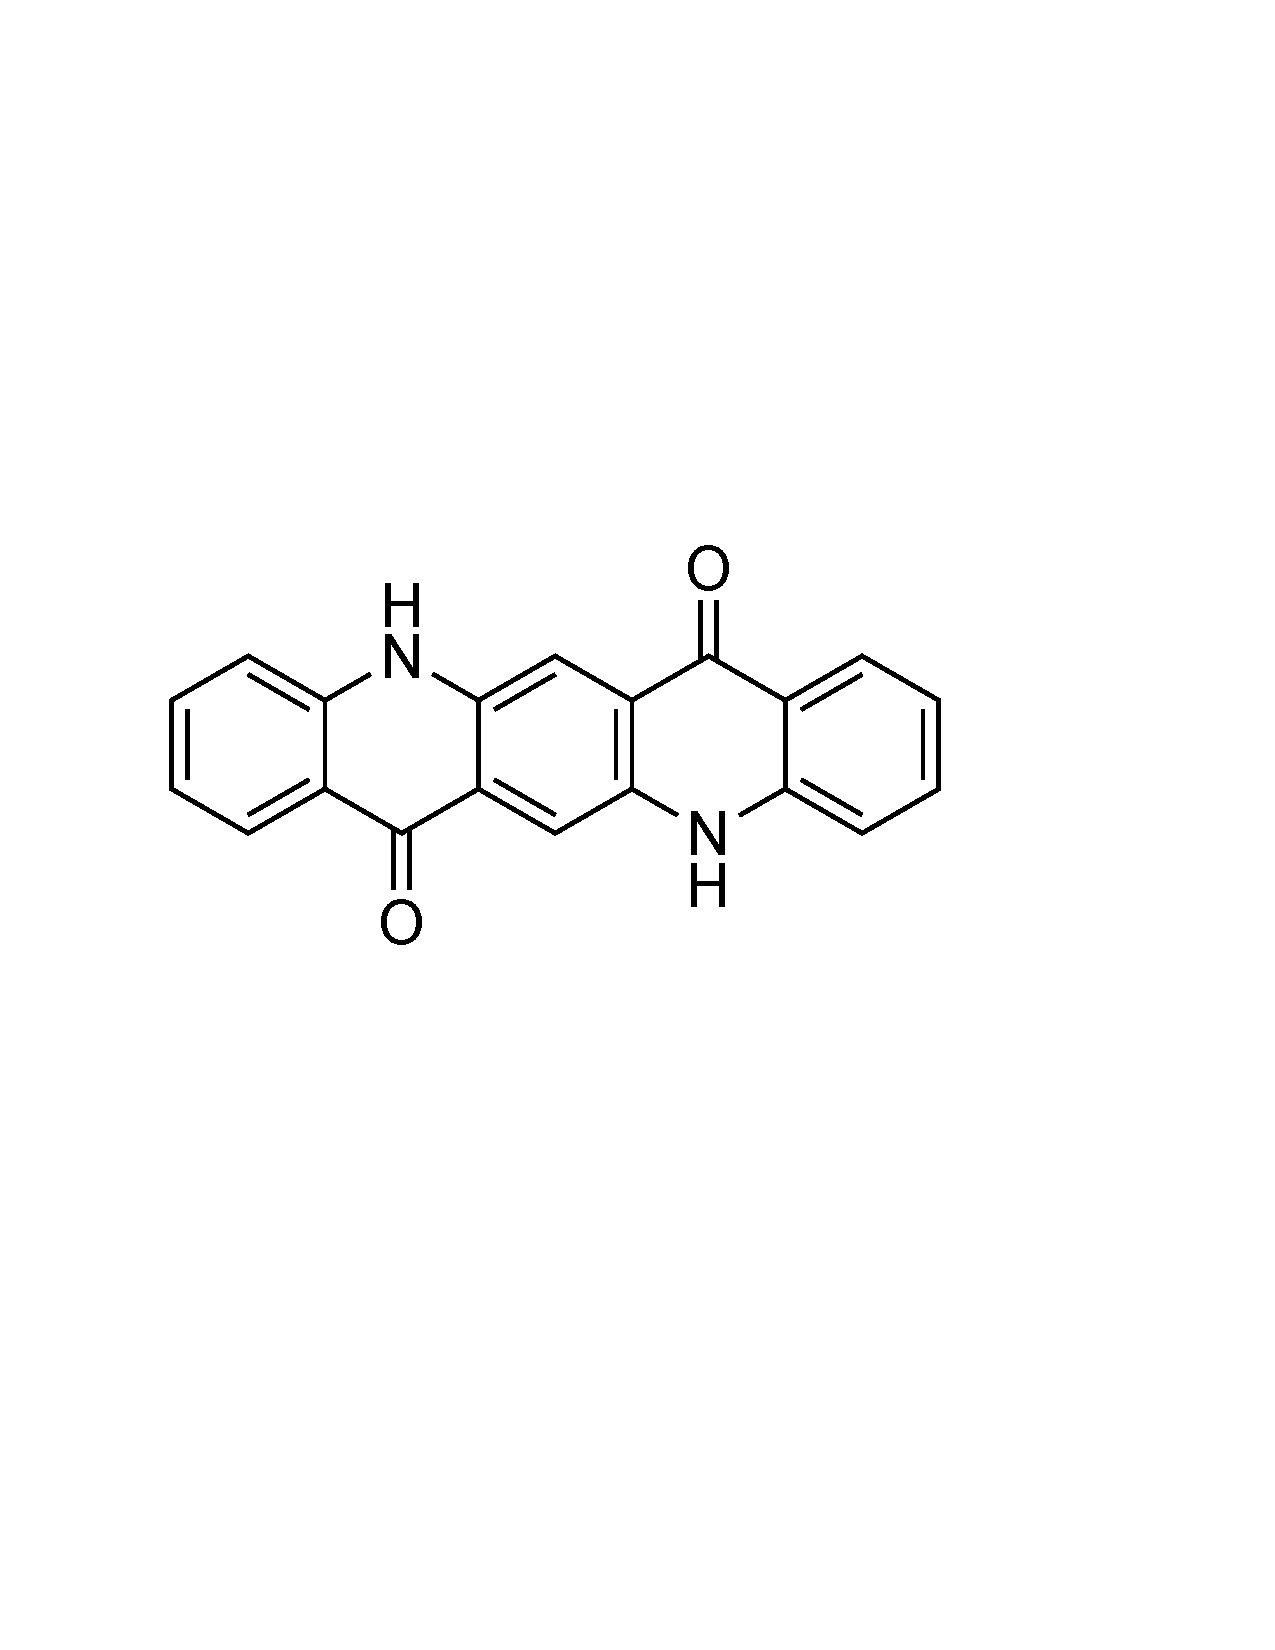
\includegraphics[width=\linewidth]{images/QA.pdf}
		\caption{Skeletal structure}
	\end{subfigure}
	\hfill
	\begin{subfigure}[b]{0.48\linewidth}
		\centering
		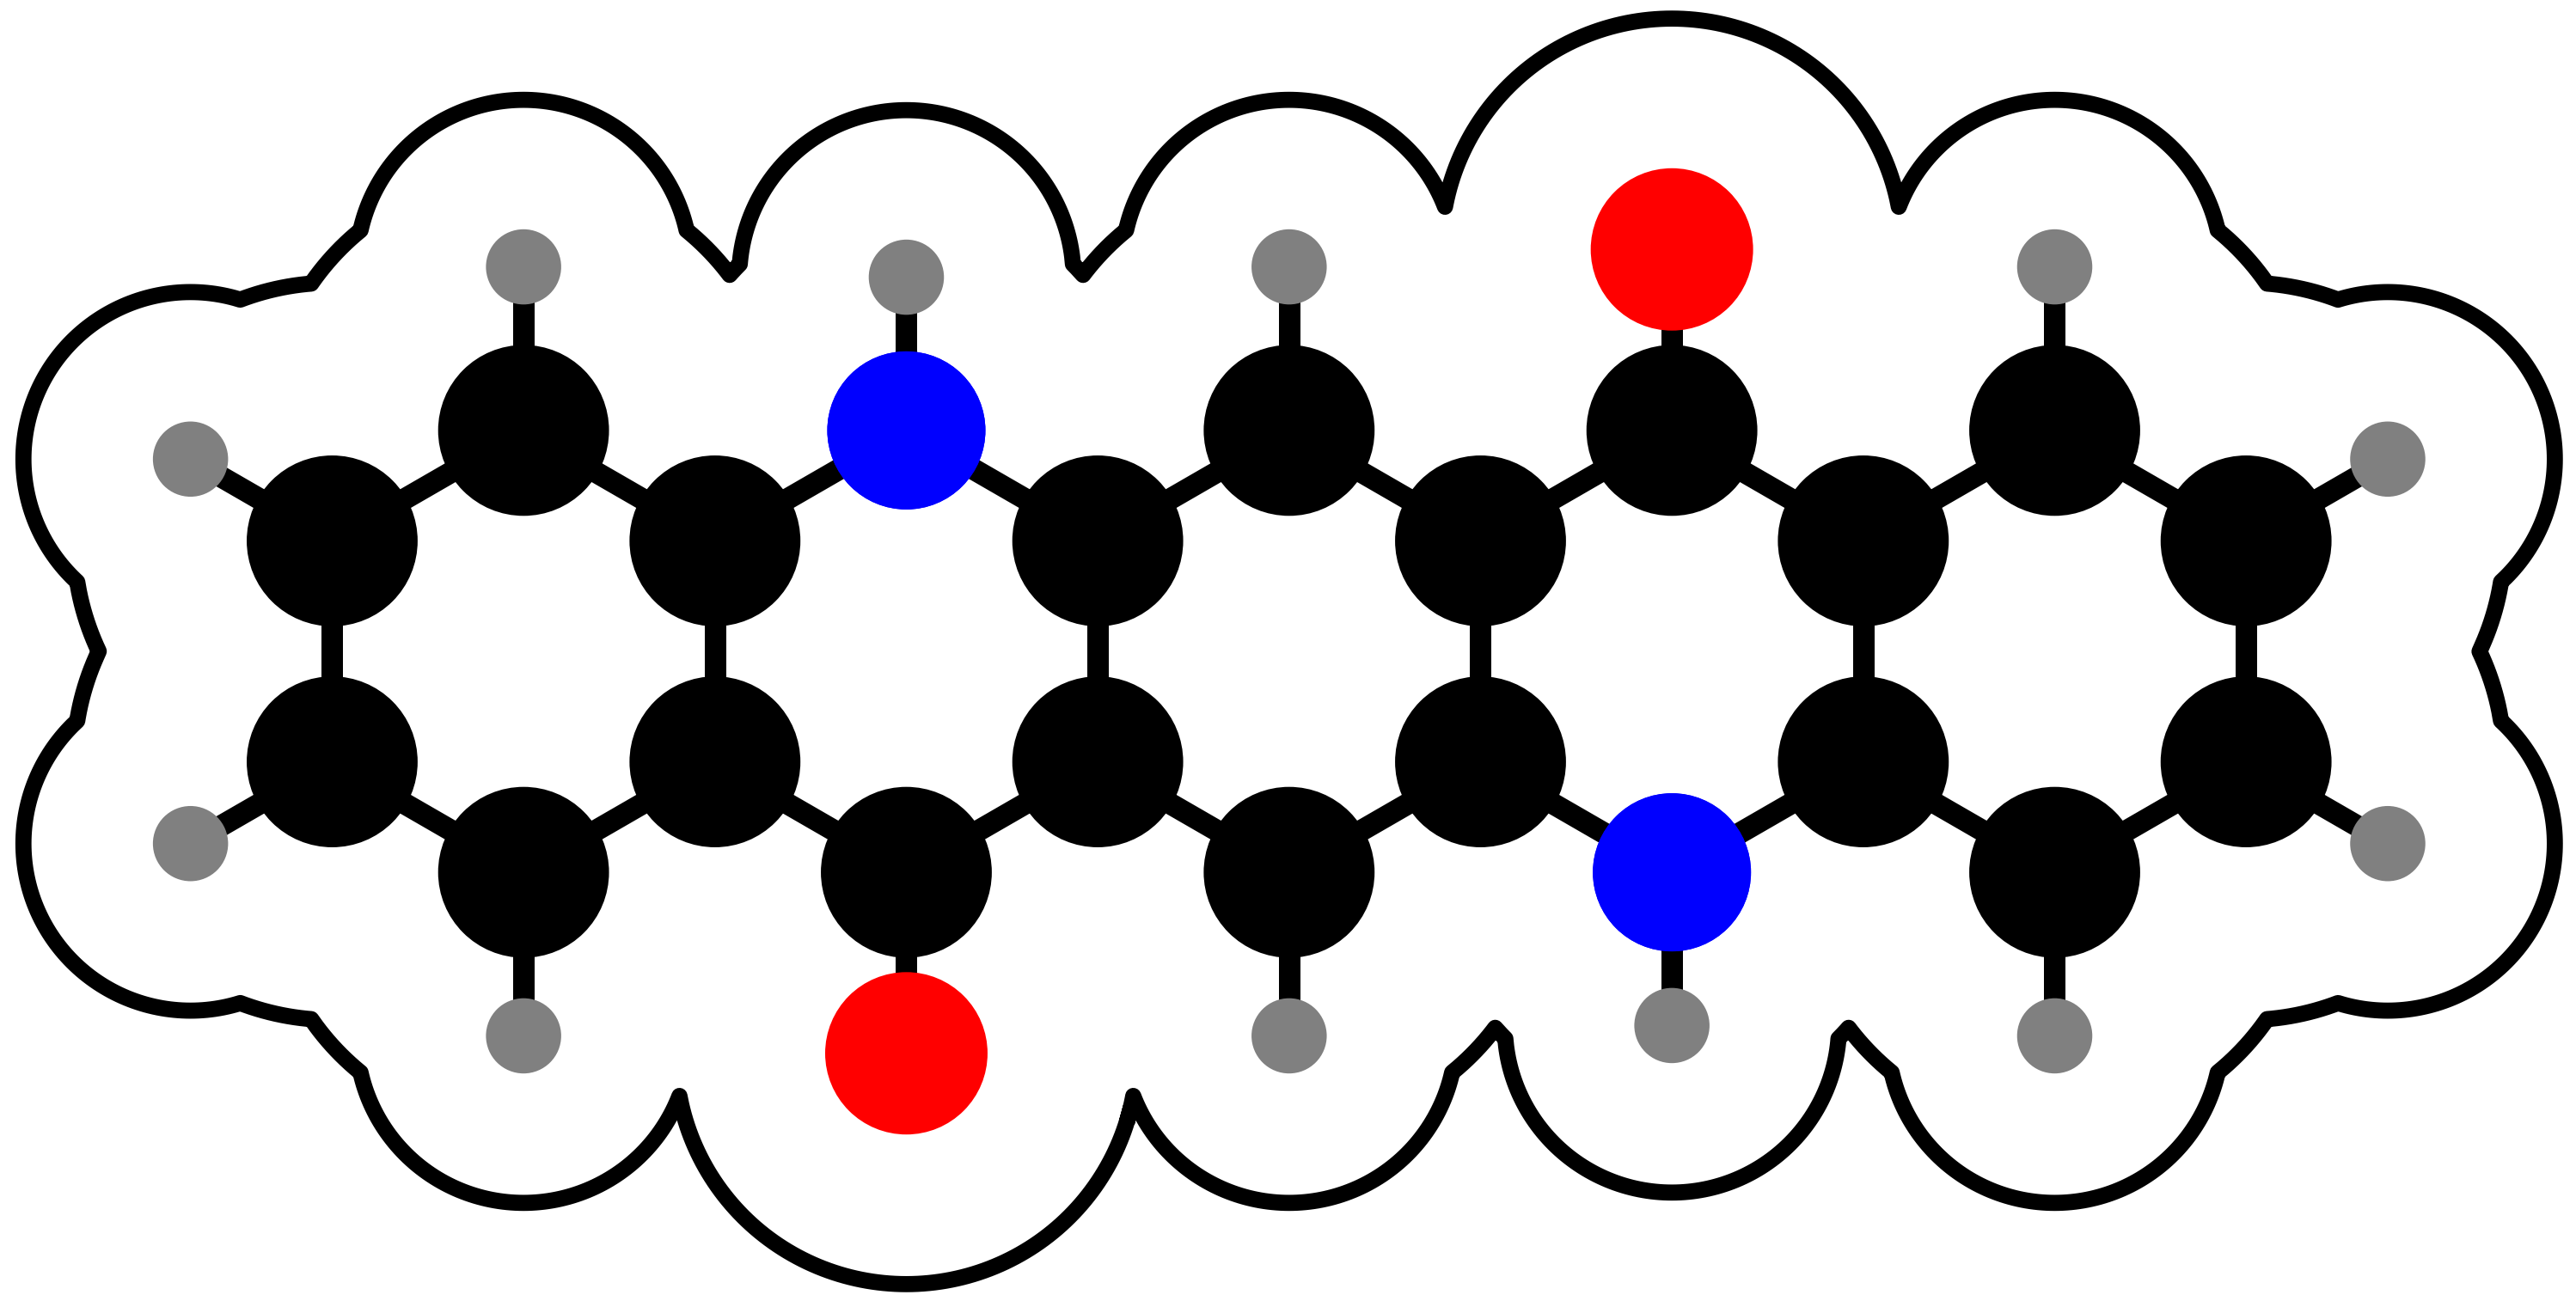
\includegraphics[width=\linewidth]{images/QA_molecule.png}
		\caption{Ball-and-stick model}
	\end{subfigure}
	\caption{Molecular structure of \acf{QA}.}
	\label{fig:QA}
\end{figure}

The molecule is classified as a heterocyclic compound. Its structure is characterized by a conjugated ring system that induces significant rigidity and planarity to the molecule.\autocite{forBiotechnologyInformation2025} \Ac{QA} is of the symmetry group $\mathrm{C_{2h}}$ and has a molar mass of 312.32~\si{g/mol}. The molecule is a crystalline solid with four known different crystal structures under standard conditions.\autocite{Paulus2007,Mizuguchi}

\newpage
\chapter{Research vision \& project idea}


\newpage
\chapter{Project milestone \& working plan for the next 6 months}

\newpage
\chapter{Appendix}
\label{sec:appendix}

\section*{List of abbreviations}
\addcontentsline{toc}{section}{List of abbreviations}
\begin{acronym}
    \acro{QA}[QA]{quinacridone}
    \acro{XPS}[XPS]{x-ray photoelectron spectroscopy}
    \acro{ML}[ML]{monolayer}
    \acro{LEED}[LEED]{low energy electron diffraction}
    \acro{UHV}[UHV]{ultra-high vacuum}
\end{acronym}

\newpage
\printbibliography[heading=bibliography]

\end{document}